\documentclass[12pt]{article}
\usepackage{graphicx}
\usepackage{amsmath}
\usepackage{mathtools}
\usepackage{gensymb}
\usepackage[utf8]{inputenc}
\usepackage{float}
\newcommand{\mydet}[1]{\ensuremath{\begin{vmatrix}#1\end{vmatrix}}}
\providecommand{\brak}[1]{\ensuremath{\left(#1\right)}}
\providecommand{\norm}[1]{\left\lVert#1\right\rVert}
\newcommand{\solution}{\noindent \textbf{Solution: }}
\newcommand{\myvec}[1]{\ensuremath{\begin{pmatrix}#1\end{pmatrix}}}
\let\vec\mathbf

\begin{document}
\begin{center}
\textbf\large{CLASS-11 \\ CHAPTER-10 \\ STRAIGHT LINES}
\end{center}
\section*{Excercise 10.4}

Q6. Find the equation of the line parallel to y-axis and drawn through the point of
intersection of the lines x – 7y + 5 = 0 and 3x + y = 0.
\section*{Solution}
The given line equations represented in vector form:
\begin{align}
\myvec{1&-7}\vec{x}&=-5\\
\myvec{3&1}\vec{x}&=0\\
\end{align}
The intersection of two lines is given by:
\begin{align}
\myvec{
1&-7&5\\
3&1&0
} \vec{x}&=0\\
\myvec{
1&-7&5\\
3&1&0
}
\xleftrightarrow[]{R_2=R_2-3R_1}
\myvec{
1&-7&5\\
0&22&-15
}\vec{x}&=0\\\xleftrightarrow[]{R_2=\frac{R_2}{22}}
\myvec{
	1&-7&5\\[1pt]
0&1&-\frac{15}{22}
}\vec{x}&=0\\
\xleftrightarrow[]{R_1={R_1}+7{R_2}}
\myvec{
1&0&\frac{5}{22}\\[1pt]
0&1&\frac{-15}{22}
}\vec{x}&=0 \label{eq:7}\\
	\vec{x}&=\myvec{-\frac{5}{22}\\[1pt] \frac{15}{22}}\\
\end{align}
To find the equation of the line parallel to the y-axis and the line passing through the $\vec{P}$ is given as
\begin{equation}
    \vec{n}^{\top}\myvec{\vec{x}-\vec{P}}=0
    \label{eq:line}
\end{equation}
Since a line is parallel to the y-axis,normal vector is in the direction of the x-axis is
\begin{equation}
    \vec{n}=\myvec{1\\0}
    \label{eq:normal}
\end{equation}
Let $\vec{P}=\myvec{-\frac{5}{22}\\[1pt] \frac{15}{22}}$ and by using \eqref{eq:line},\eqref{eq:direction} and \eqref{eq:normal}
\begin{align}
    \myvec{1&0}\myvec{\vec{x}-\myvec{-\frac{5}{22}\\[1pt] \frac{15}{22}}}=0\\
    \myvec{1&0}\vec{x}=-\frac{5}{22}
\end{align}
\begin{figure}[H]
	\begin{center} 
	    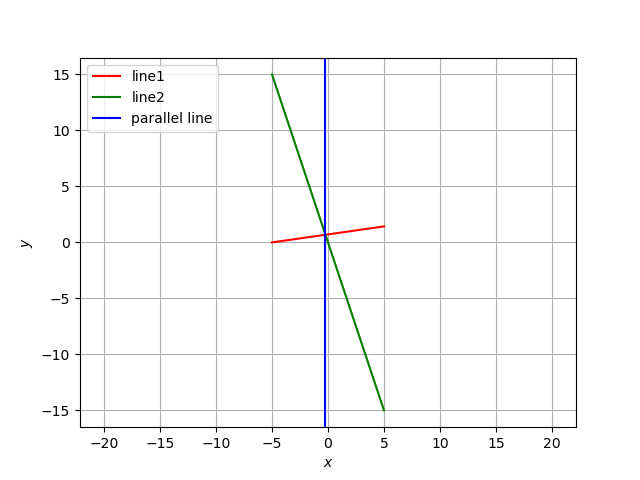
\includegraphics[width=\columnwidth]{figs/line.png}
	\end{center}
\caption{}
\label{fig:Fig3}
\end{figure}
\end{document}
